% --- SECCIÓ 2: MARC TEÒRIC ---
\apartat{Marc Teòric}

\subsection{La Comunicació Humana i el seu Processament}
La comunicació és un procés complex i multidimensional que permet als éssers humans intercanviar informació, expressar emocions i construir relacions socials. Des d'una perspectiva neuropsicològica, la comunicació requereix la integració de múltiples àrees cerebrals, especialment l'àrea de Broca i l'àrea de Wernicke\footnote{L'àrea de Broca s'encarrega de la producció del llenguatge, mentre que l'àrea de Wernicke és fonamental per a la comprensió del mateix.}, que gestionen tant el contingut com la forma del missatge.

% --- ESQUEMA TÈCNIC: COMPONENTS DE LA COMUNICACIÓ ---
\begin{figure}[ht]
    \centering
    \begin{tikzpicture}[node distance=1.5cm, auto,
        block/.style={rectangle, draw, fill=MidnightBlue!10, text width=8em, text centered, rounded corners, minimum height=3.5em, font=\small, drop shadow},
        line/.style={draw, -latex', MidnightBlue, thick}]
        
        \node [block, fill=MidnightBlue!25] (com) {\textbf{Estructura de la Comunicació}};
        \node [block, below left=1.5cm and 0.2cm of com] (verb) {Component Verbal\\(Semàntica i Sintaxi)};
        \node [block, below=2cm of com] (noverb) {Component No Verbal\\(Cinèsica i Proxèmica)};
        \node [block, below right=1.5cm and 0.2cm of com] (caa) {CAA\\(Suport Multimodal)};
        
        \path [line] (com) -- (verb);
        \path [line] (com) -- (noverb);
        \path [line] (com) -- (caa);
    \end{tikzpicture}
    \caption{Representació gràfica de les dimensions comunicatives abordades en el treball.}
\end{figure}

\newpage
\subsection{Comunicació Augmentativa i Alternativa (CAA)}
\begin{tcolorbox}[colback=TealBlue!5, colframe=TealBlue, arc=5pt, title=La CAA com a eina d'inclusió, fonttitle=\bfseries, shadow={2pt}{-2pt}{0pt}{black!10}]
    La CAA engloba tot aquell conjunt d'estratègies que busquen maximitzar les capacitats comunicatives. Segons l'ISAAC\footnote{International Society for Augmentative and Alternative Communication.}, l'objectiu no és només parlar, sinó permetre la participació plena en la societat.
\end{tcolorbox}

% --- TAULA COMPARATIVA DE SISTEMES ---
\begin{table}[ht]
    \centering
    \small
    \begin{tabular}{@{} l p{3.5cm} c c c @{}}
    \toprule
    \textbf{Sistema} & \textbf{Descripció} & \textbf{Portabilitat} & \textbf{Càrrega Cognitiva} & \textbf{Autonomia} \\
    \midrule
    \rowcolor{gray!5} ARASAAC & Pictogrames gratuïts & \cmark & Baixa & Alta \\
    SPC & Símbols clàssics & \cmark & Baixa & Mitjana \\
    \rowcolor{gray!5} DCOV & Dispositius amb veu & \xmark & Alta & Molt Alta \\
    \bottomrule
    \end{tabular}
    \caption{Anàlisi comparatiu de les solucions de suport segons criteris tècnics.}
\end{table}

\subsection{Integració Sensorial: Fonaments i Impacte}
La integració sensorial és el procés neurològic d'organitzar les sensacions per al seu ús. Segons la piràmide d'aprenentatge de Williams i Shellenberger\footnote{Model que explica com el desenvolupament sensorial és la base de les habilitats cognitives i acadèmiques.}, la regulació dels sentits és el fonament de tot creixement acadèmic.

% --- ESQUEMA TIKZ: PIRÀMIDE SENSORIAL ---
\begin{figure}[ht]
    \centering
    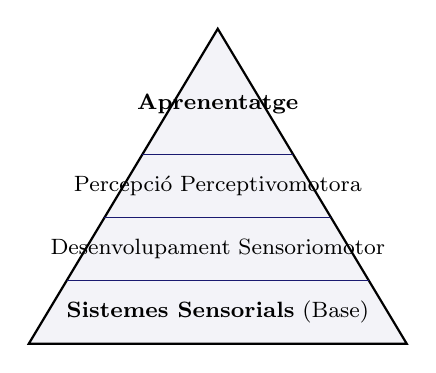
\begin{tikzpicture}[scale=0.8]
        \draw[thick, fill=MidnightBlue!5] (0,0) -- (6,0) -- (3,5) -- cycle;
        \draw[MidnightBlue] (0.6,1) -- (5.4,1);
        \draw[MidnightBlue] (1.2,2) -- (4.8,2);
        \draw[MidnightBlue] (1.8,3) -- (4.2,3);
        
        \node at (3,0.5) {\footnotesize\textbf{Sistemes Sensorials} (Base)};
        \node at (3,1.5) {\footnotesize Desenvolupament Sensoriomotor};
        \node at (3,2.5) {\footnotesize Percepció Perceptivomotora};
        \node at (3,3.8) {\footnotesize\textbf{Aprenentatge}};
    \end{tikzpicture}
    \caption{Piràmide simplificada de la integració sensorial en el desenvolupament.}
\end{figure}

La taula sensorial actua en la base d'aquesta piràmide, oferint estímuls tàctils i visuals que preparen el cervell per a processos superiors com el llenguatge.

\subsection{Dificultats Comunicatives Específiques}
\begin{itemize}
    \item \textbf{TEA (Trastorn de l'Espectre Autista):} Presenten dificultats en la comunicació social. La regulació sensorial mitjançant llums i textures pot reduir l'estrès ambiental.
    \item \textbf{Paràlisi Cerebral:} Afecta l'execució motora. La taula sensorial ofereix una via d'interacció que no depèn de la motricitat fina.
    \item \textbf{Retard maduratiu:} L'estimulació multisensorial accelera la creació de connexions neuronals (neuroplasticitat).
\end{itemize}
